\documentclass[parskip=half, bibliography=totoc, captions=tableheading]{scrartcl} %Ich habe [parskip=half] hinzugefügt

%\usepackage[calc]{picture}
\usepackage{fixltx2e}

\usepackage{tcolorbox}

%\pagestyle{headings}
\usepackage[headtopline,headsepline]{scrpage2}
\setheadsepline{.5pt}
\pagestyle{scrheadings}
\cfoot[\pagemark]{\pagemark}
%\ihead{\headmark}
%\ihead{\headmark}
\ohead{16. Dezember 2016}
\automark{section}


\usepackage{polyglossia}
\setmainlanguage{german}
\usepackage{caption}
\usepackage{amsmath}
\usepackage{amssymb}
\usepackage{mathtools}

\usepackage{fontspec}
\defaultfontfeatures{Ligatures=TeX}

\usepackage[
  math-style=ISO,
  bold-style=ISO,
  sans-style=italic,
  nabla=upright,
]{unicode-math}

\setmathfont{Latin Modern Math}
%\setmathfont[range={\mathscr, \mathbfscr}]{XITS Math}
%\setmathfont[range=\coloneq]{XITS Math}
%\setmathfont[range=\propto]{XITS Math}

\usepackage[autostyle]{csquotes}

\usepackage[
  locale=DE,                   % deutsche Einstellungen
  separate-uncertainty=true,   % Immer Fehler mit \pm
  per-mode=symbol-or-fraction, % m/s im Text, sonst Brüche
]{siunitx}
%\sisetup{math-stylemicro=\text{µ},text-micro=µ}

\usepackage{xfrac}

\usepackage[section, below]{placeins}
\usepackage[
  labelfont=bf,
  font=small,
  width=0.9\textwidth,
]{caption}

\usepackage{subcaption}

\usepackage{graphicx}

\usepackage{float}
\floatplacement{figure}{h}
\floatplacement{table}{h}

\usepackage{booktabs}



\usepackage{bookmark}

\usepackage[shortcuts]{extdash}

\usepackage[math]{blindtext}

\usepackage{microtype}

\usepackage[
  backend=biber,
]{biblatex}
% Quellendatenbank
\addbibresource{lit.bib}

\usepackage{hyperref}

\usepackage{color} % Das ist Geschmacksfrage

\usepackage{makeidx} %Ich habe makeidx hinzugefügt + makeindex
\makeindex


\usepackage[version=3]{mhchem} % für Thermodynamik-chemische Elemente
\usepackage{enumitem} %Ich habe enumitem hinzugefügt
\usepackage{expl3}
\usepackage{xparse}
%\ExplSyntaxOn

\NewDocumentCommand \dif {m}
{
\mathinner{\symup{d} #1}
}
\usepackage{subcaption}


%\usepackage{showframe}
\author{Steven Becker \\
steven.becker@tu-dortmund.de \\
und \\
Stefan Grisard \\
stefan.grisard@tu-dortmund.de}

\title{Tutorium Experimentelle Physik I}
%\subtitle{}

\date{\today}

\begin{document}

\frame{\maketitle}

\section{1. Teil}
\begin{frame}{Blindtext}
\blindtext

\end{frame}

\begin{frame}{Mehrere Spalten}
\begin{columns}[onlytextwidth]
\begin{column}{0.45\textwidth}
\blindlist{enumerate}[6]
\end{column}
\begin{column}{0.45\textwidth}
  \pause
\blindlist{itemize}[6]
\end{column}
\end{columns}
\end{frame}

\section{2. Teil}
\begin{frame}{oxford Blöcke}
\begin{block}{Erster Block}
\begin{itemize}
  \item hier ein paar Stichpunkte
\end{itemize}
\end{block}
\begin{exampleblock}{Anderer Block}
Hier pipapo
\end{exampleblock}
\begin{alertblock}{Gewagter Block}
Hallihallo, jah f ahd jalkjs aksjd alkjs fgoiho iwqfkalf.
\end{alertblock}
\end{frame}

\begin{frame}{Formeln}
\begin{equation}
  \int_{0}^{1}  (x^2 + 2x)\mathup{d}\, x = \left. \frac{1}{3}x^3 + x^2\right|_0^{1} = \frac{4}{3}
\end{equation}
\begin{equation}
  \int_{0}^{1}  (x^2 + 2x)\mathup{d}\, x = \left. \frac{1}{3}x^3 + x^2\right|_0^{1} = \frac{4}{3}
\end{equation}
\begin{equation}
  \int_{0}^{1}  (x^2 + 2x)\mathup{d}\, x = \left. \frac{1}{3}x^3 + x^2\right|_0^{1} = \frac{4}{3}
\end{equation}
\end{frame}

\begin{frame}{Bilder}

\begin{figure}
  \centering
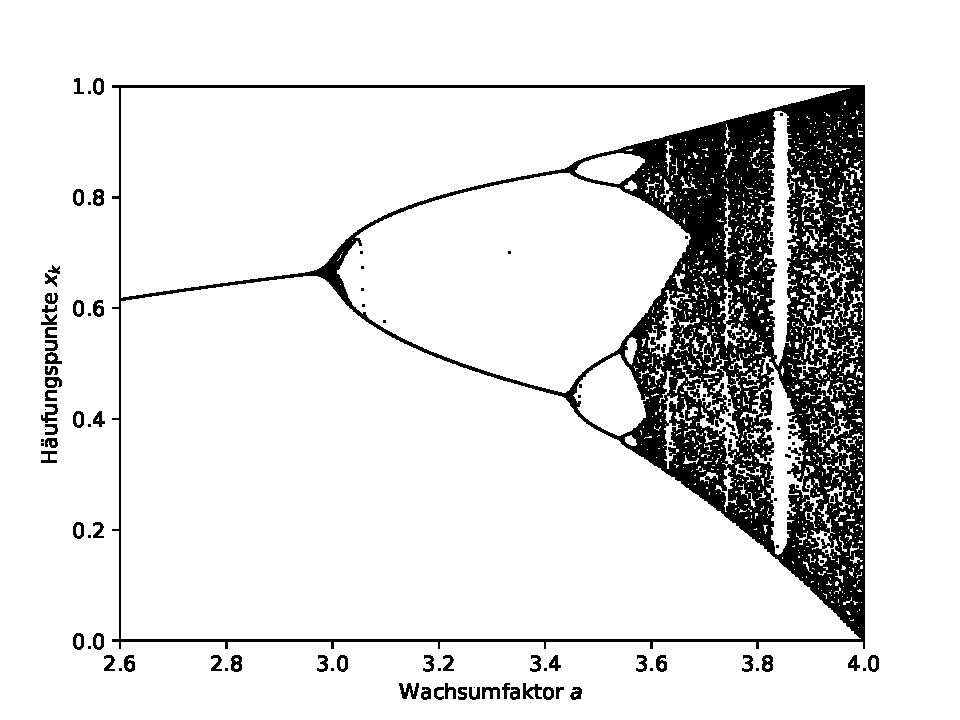
\includegraphics[width=0.7\textwidth]{feigenbaumdiagramm.pdf}
  \caption{TestBild mit Test-Caption}
  \label{fig: testfigure}
\end{figure}


\end{frame}

\end{document}
